\subsection{Improve workflow with branching}
Up to this point, only some basic activities of the version control software have been
demonstrated like saving changes to the project files and displaying history of changes. No branching
has been done, however, it is more important feature when it comes to complex development project, faster iteration cycles and
CI/CD principles. In this section, a new development branch (stream in Perforce's terminology) is created beside the one
called main and all incremental development is done to the development branch which is later merged to the main one.
\subsubsection{Setup new stream}
steps to setup streams in Perforce
\begin{figure}[H]
    \centering
    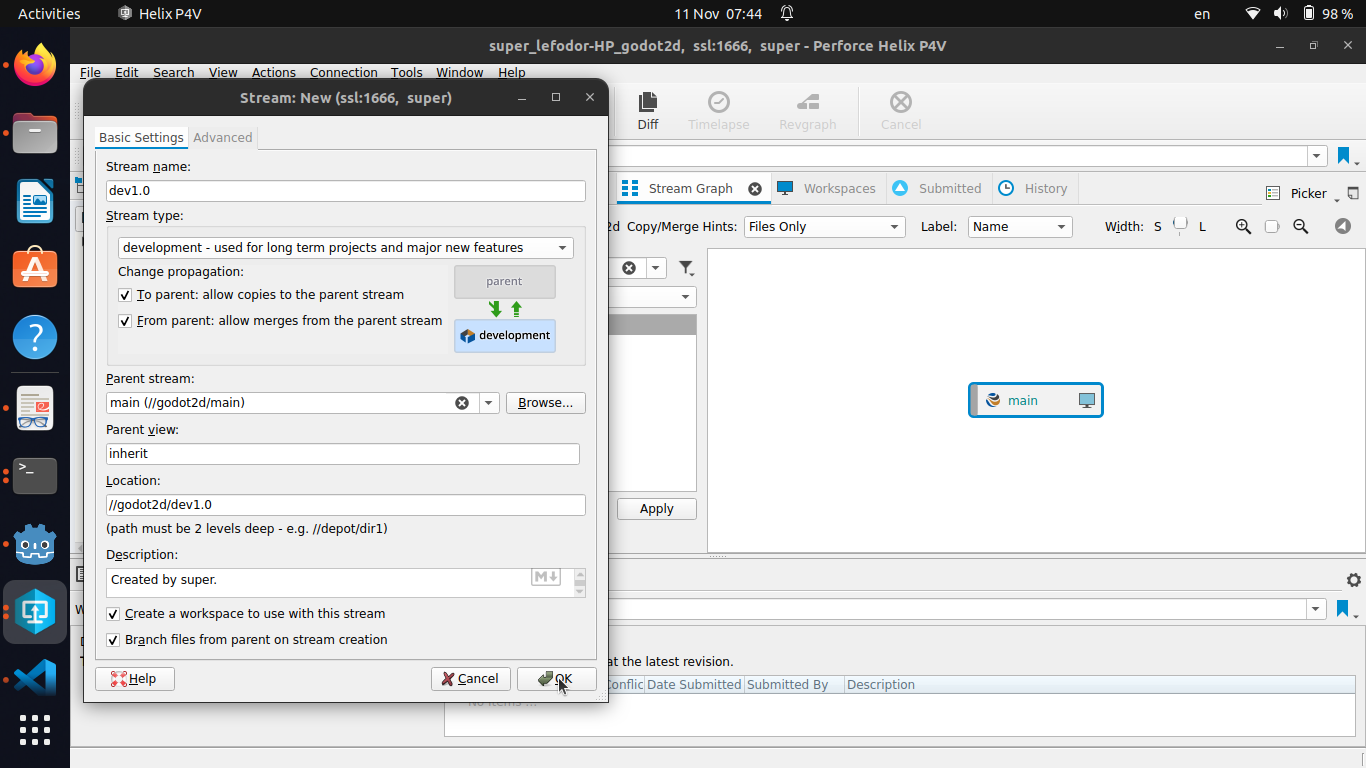
\includegraphics[width=\textwidth]{new-stream-for-branching.png}
      \caption{p4v new stream for branching}
      \label{fig:new-stream-for-branching}
\end{figure}
A new development stream (branch) has been created:
\begin{figure}[H]
    \centering
    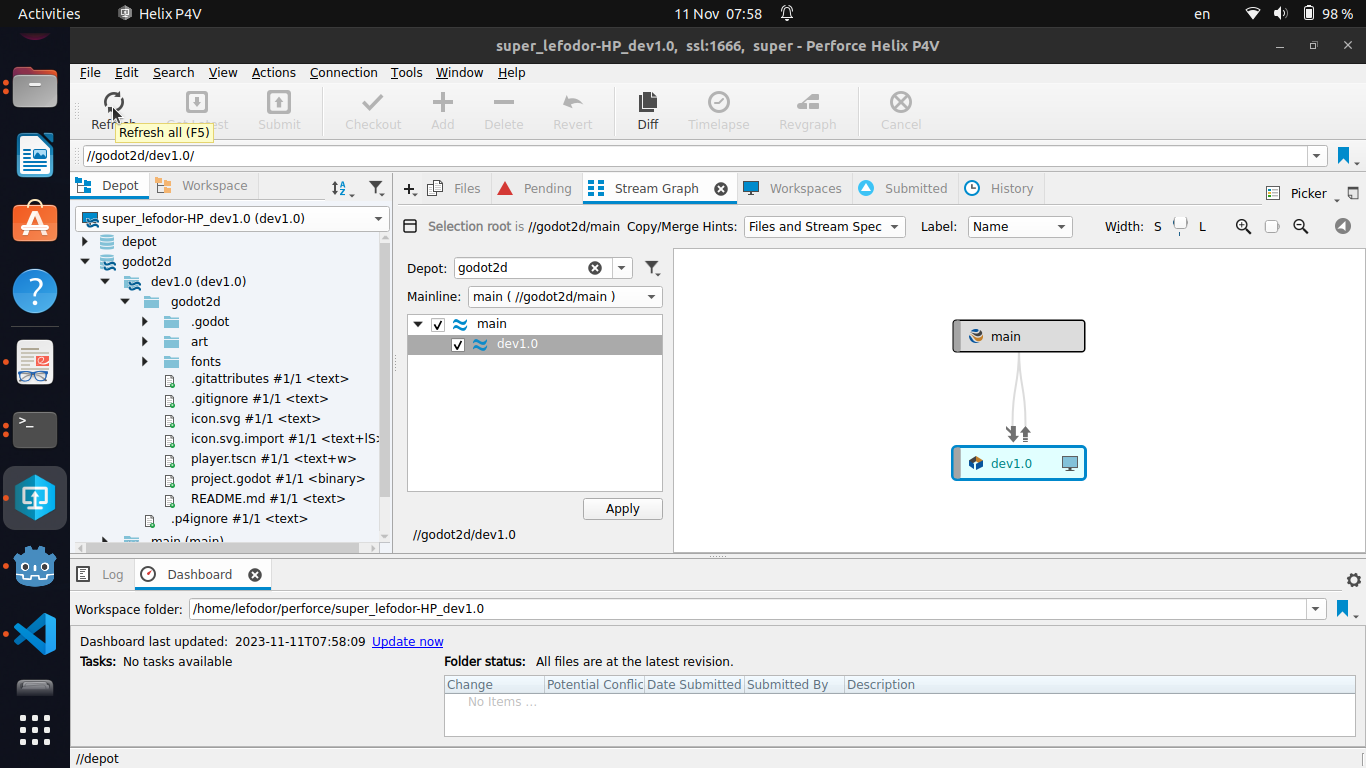
\includegraphics[width=\textwidth]{new-branch-dev1.0.png}
      \caption{new stream (branch) dev1.0}
      \label{fig:new-branch-dev1.0}
\end{figure}
From this point onwards, all changes are to be made on the development stream and later merged back to the more stable
main stream. Also, changes need to be made to the workspace related to this branch and not on the one linked to main.

\subsection{Development steps cont'd}
\begin{enumerate}[resume]
  \item \href{https://docs.godotengine.org/en/stable/getting_started/first_2d_game/03.coding_the_player.html}{\color{blue}Coding player scene}. 
  Add script to player scene. Check for input, move in direction, play the animation related
  to the movement.
  Add script to player by selecting the scene and click on the "Attach Script" button.
  \begin{figure}[H]
    \centering
    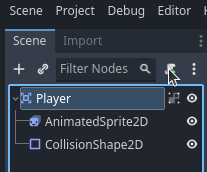
\includegraphics[scale=0.5]{add-script-to-player.png}
      \caption{add script to player}
      \label{fig:add-script-to-player}
  \end{figure}
  The added script (\textit{player.gd}) should look like as below:
  \begin{verbatim}
    extends Area2D

    @export var speed = 400 # How fast the player will move (pixels/sec).
    var screen_size # Size of the game window.
    
    # Called when the node enters the scene tree for the first time.
    func _ready():
      screen_size = get_viewport_rect().size
    
    
    # Called every frame. 'delta' is the elapsed time since the previous frame.
    func _process(delta):
      var velocity = Vector2.ZERO # The player's movement vector.
      if Input.is_action_pressed("ui_right"):
        velocity.x += 1
      if Input.is_action_pressed("ui_left"):
        velocity.x -= 1
      if Input.is_action_pressed("ui_down"):
        velocity.y += 1
      if Input.is_action_pressed("ui_up"):
        velocity.y -= 1
    
      if velocity.length() > 0:
        velocity = velocity.normalized() * speed
        $AnimatedSprite2D.play()
      else:
        $AnimatedSprite2D.stop()
      
      if velocity.x != 0:
        $AnimatedSprite2D.animation = "walk"
        $AnimatedSprite2D.flip_v = false
        # See the note below about boolean assignment.
        $AnimatedSprite2D.flip_h = velocity.x < 0
      elif velocity.y != 0:
        $AnimatedSprite2D.animation = "up"
        $AnimatedSprite2D.flip_v = velocity.y > 0
      
      position += velocity * delta
      position = position.clamp(Vector2.ZERO, screen_size)    

  \end{verbatim} 
  After this step, it is already possible to run the game by pressing F6 and use the arrow buttons to control the player's
  character up/down and left/right.
\end{enumerate}